\documentclass[a4paper, 12pt]{article}
\usepackage[utf8]{inputenc}
\usepackage[english]{babel}
\usepackage{graphicx}
\usepackage{hyperref}
\usepackage[a4paper]{geometry}
\usepackage{movie15}
%\usepackage[left=1cm,right=2cm,vmargin=2.5cm,footnotesep=0.5cm]{geometry}
\usepackage{amssymb,amsmath,amsthm}
\DeclareMathOperator*{\E}{\mathbb{E}}
\DeclareMathOperator*{\Var}{\text{Var}}
\renewcommand*{\P}{\mathbb{P}}
\newtheorem{theorem}{Theorem}
\newtheorem{lemma}{Lemma}

\hypersetup{
    colorlinks=true,
    linkcolor=blue,
    filecolor=magenta,      
    urlcolor=cyan,
    pdftitle={Sharelatex Example},
    bookmarks=true,
    pdfpagemode=FullScreen
}

  
\begin{document} 

\begin{titlepage}
	\centering
	{\scshape\LARGE Ozonmasters \par}
	\vspace{1cm}
	{\scshape\Large Statistics \par}
	\vspace{1.5cm}
	{\huge\bfseries Home work \par}
	\vspace{2cm}
	{\Large\itshape Kozhemyak Vitaly \par}
	\vfill

% Bottom of the page
	{\large \today\par}
\end{titlepage}
  
\tableofcontents

\newpage
\section{Task 1}
\subsection{Theoretical solution}
The next functional in kernel $K:$
$$
J(K) = \left( \int \limits_{- \infty}^{+\infty} K^2(x)dx \right) \left( \int \limits_{- \infty}^{+\infty} x^2 K(x)dx \right)^{1/2}
$$
is called \textit{kernel efficiency.}
\begin{enumerate}
	\item Consider $K_1(x) = \mathbb{I}[x \in [-1/2, 1/2]].$ Then
$$
J(K_1) = \left( \int \limits_{- 1/2}^{+1/2} dx \right) \left( \int \limits_{- 1/2}^{+1/2} x^2 dx \right)^{1/2} = \left( \dfrac{1}{12} \right)^{1/2}.
$$
	\item Consider $K_2(x) = \dfrac{1}{\sqrt{2 \pi}} e^{-\frac{x^2}{2}}.$ Then
$$
J(K_2) = \left( \dfrac{1}{2 \pi} \int \limits_{- \infty}^{+\infty} e^{-x^2} dx \right) \left( \dfrac{1}{\sqrt{2 \pi}} \int \limits_{- \infty}^{+ \infty} x^2 e^{-\frac{x^2}{2}} dx \right)^{1/2} = \dfrac{1}{2 \sqrt{\pi}}.
$$
	\item Consider $K_{ep}(x) = \dfrac{3}{4} (1 - x^2) \mathbb{I}[|x| \leqslant 1].$ Then
	$$
J(K_{ep}) = \left( \dfrac{9}{16} \int \limits_{- 1}^{1} (1-x^2)^2 dx \right) \left( \dfrac{3}{4} \int \limits_{-1}^{1} x^2 (1-x^2) dx \right)^{1/2} = \dfrac{3}{5 \sqrt{5}}.
$$
\end{enumerate}
Let's calculate efficiency relative to the Epanechnikov kernel
\begin{itemize}
	\item For $K_1(x)$ it's $\dfrac{J(K_{ep})}{J(K_1)} \cdot 100\% = 92.9\%;$
	\item For $K_2(x)$ it's $\dfrac{J(K_{ep})}{J(K_2)} \cdot 100\% = 95.1\%.$
\end{itemize}
\subsection{Numerical solution}
The next picture shows us the water rate distribution using Sturges estimator
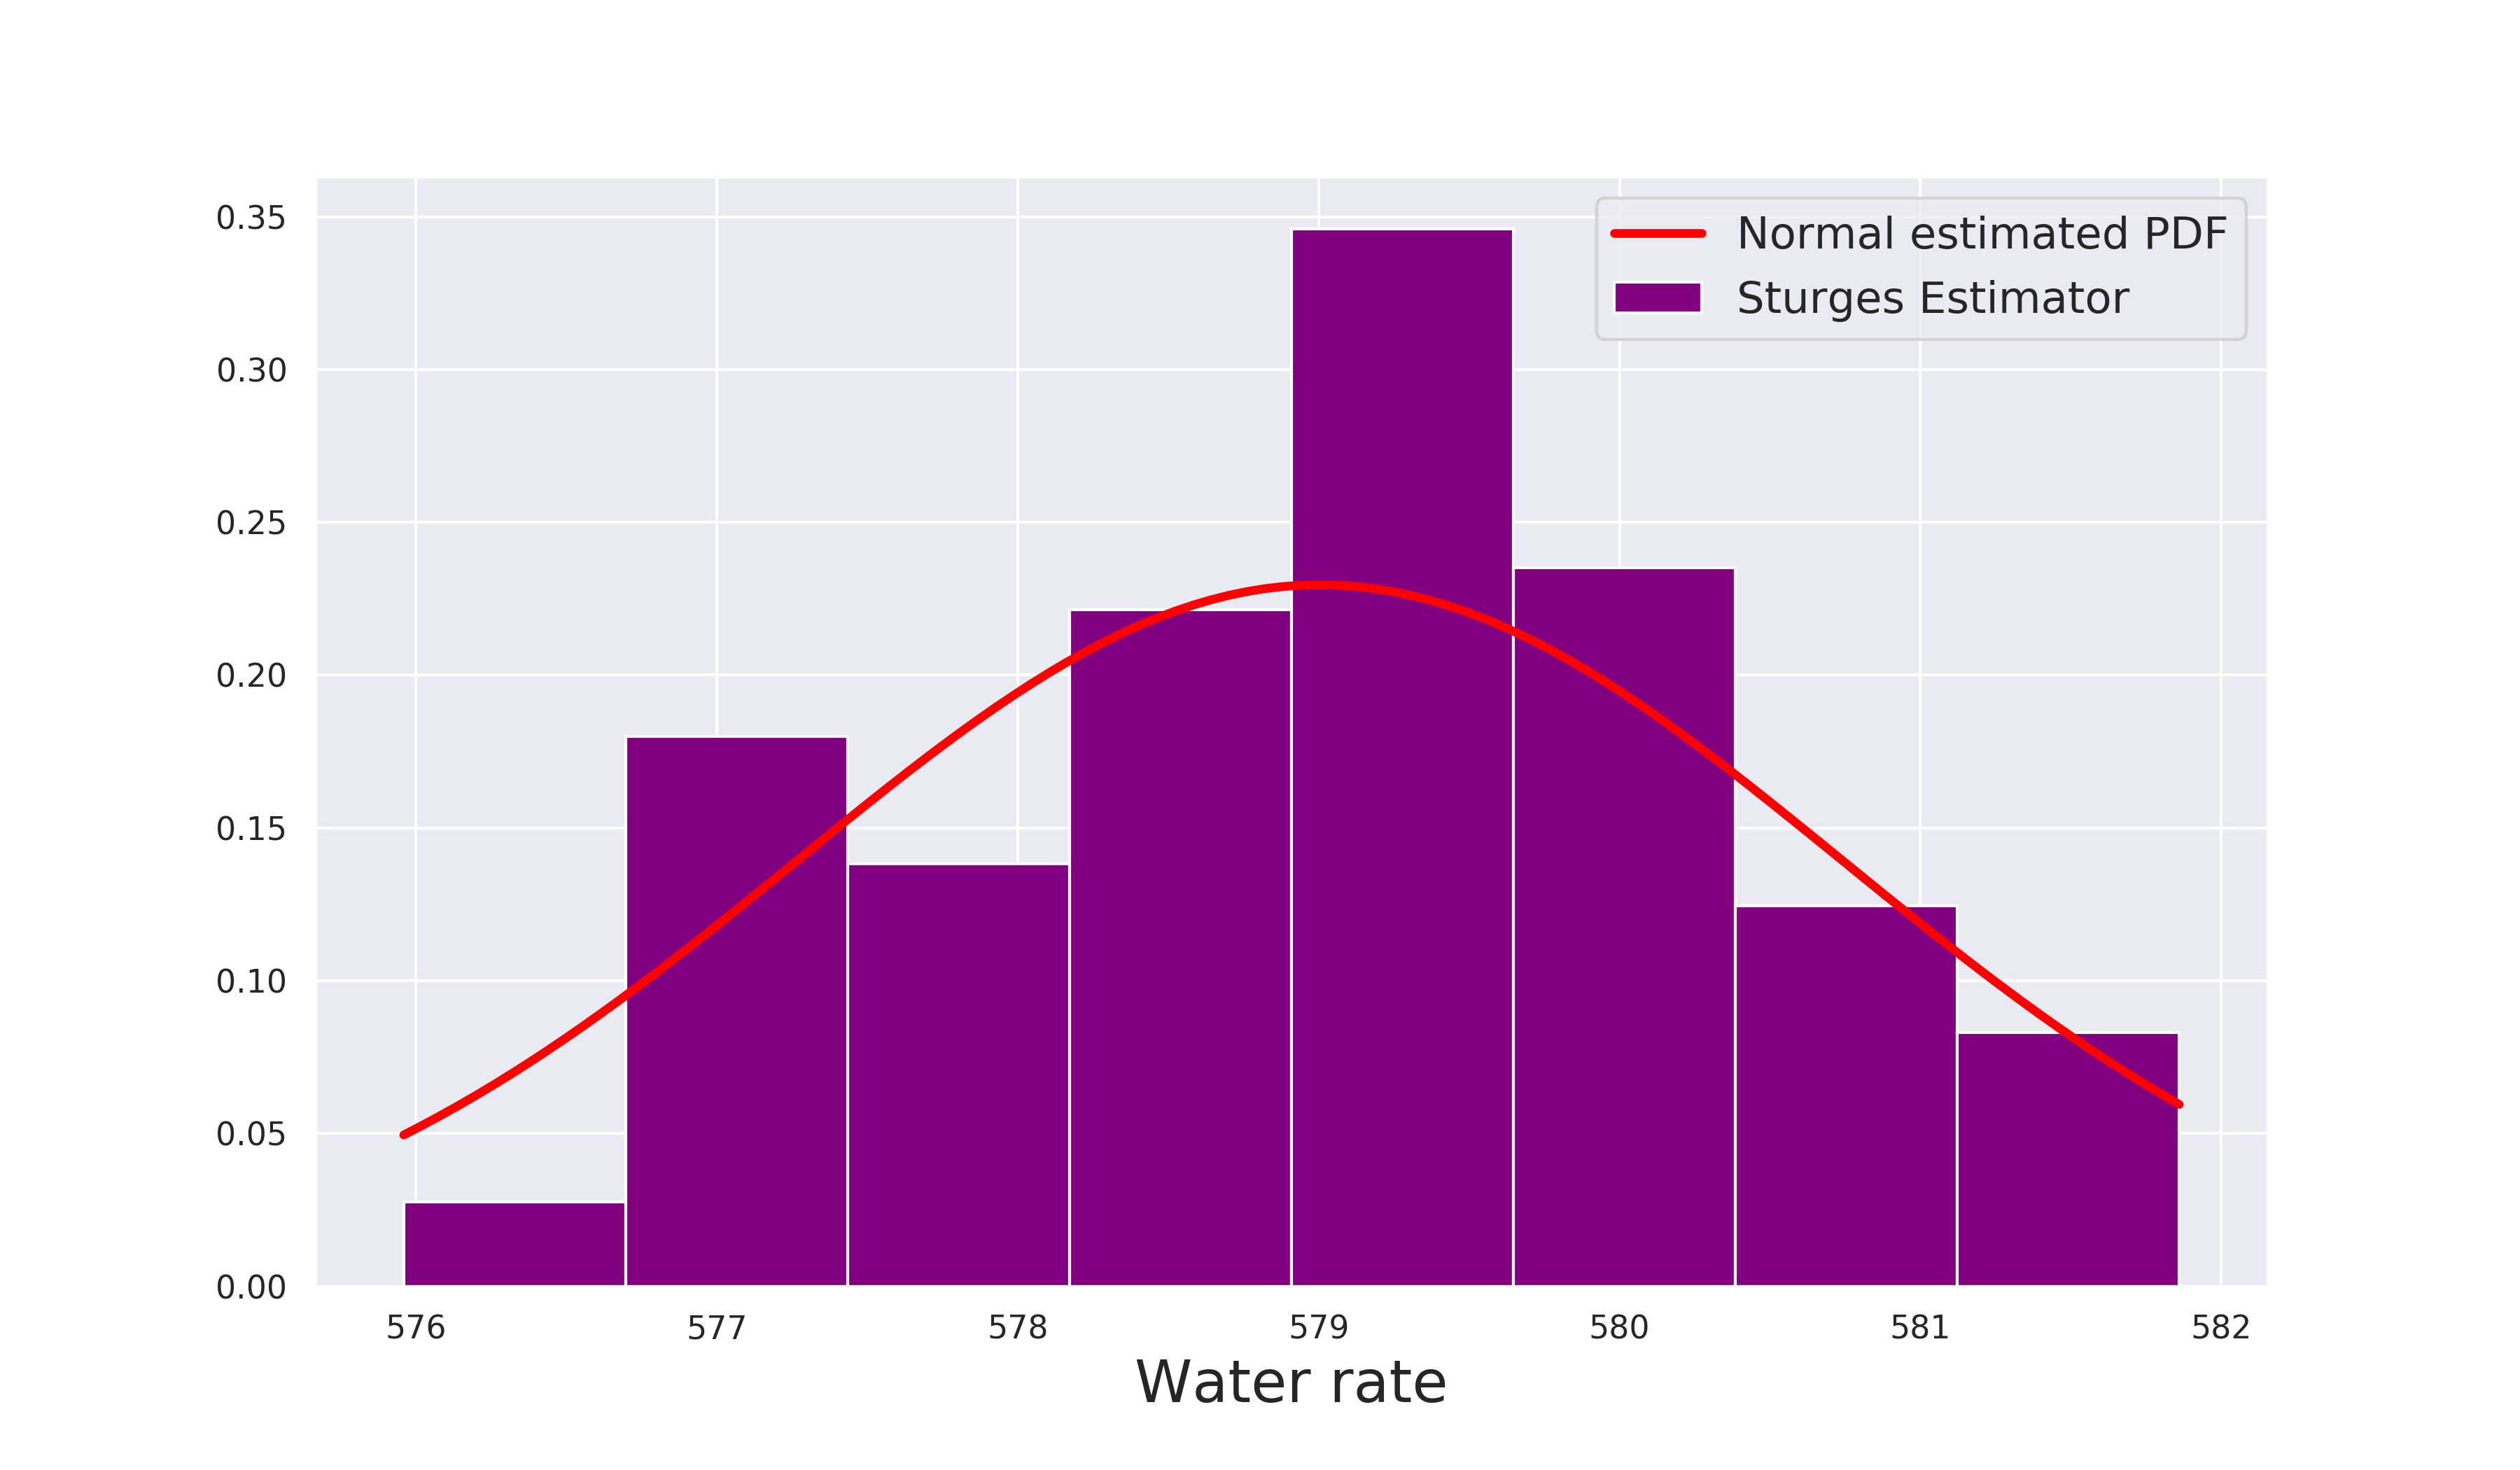
\includegraphics[width=\textwidth]{Images/Task1_1.png}

To show the bias-variance trade off you should  visit the next \href{https://github.com/vitomania/ozon/blob/master/stats/hw2/Images}{link} and download file named \texttt{Task1\_2.gif} which is represented GIF-animation.


\section{Task 2}
\subsection{Theoretical solution}
Suppose we have random variable $X$ drawn from distribution with the density function 
\begin{equation}
\label{eq2_1}
p(x) = \dfrac{1}{2} \mathcal{N}(x; 0, 1) + \dfrac{1}{4} \mathcal{E}(x+2; 1) + \dfrac{1}{4} \mathcal{E}(-x+2; 1).
\end{equation}
\paragraph{Expected value.} According to the definition of expected value
$$
\E [X] = \int \limits_{- \infty}^{+\infty} x p(x) dx = \dfrac{1}{2} \dfrac{1}{\sqrt{2 \pi}} \int \limits_{-\infty}^{+\infty} xe^{-\frac{1}{2}x^2} dx + \dfrac{1}{4} \int \limits_{-2}^{+\infty} xe^{-(x+2)} dx + \dfrac{1}{4} \int \limits_{-\infty}^{2} xe^{-(-x+2)} dx = 0.
$$
\paragraph{Variance.} According to the definition of variance
$$
\Var [X] = \E [X^2] - (\E [X])^2 = \E[X^2] = 
$$
$$
= \int \limits_{- \infty}^{+\infty} x^2 p(x) dx = \dfrac{1}{2} \dfrac{1}{\sqrt{2 \pi}} \int \limits_{-\infty}^{+\infty} x^2e^{-\frac{1}{2}x^2} dx + \dfrac{1}{4} \int \limits_{-2}^{+\infty} x^2e^{-(x+2)} dx + \dfrac{1}{4} \int \limits_{-\infty}^{2} x^2e^{-(-x+2)} dx =
$$
$$
= \dfrac{1}{2} + 1 + 1 = \dfrac{5}{2}.
$$
\paragraph{Characteristic function.}
According to the definition of characteristic function
$$
\varphi_X(t) = \E e^{itX} = 
$$
$$
= \int \limits_{- \infty}^{+\infty} e^{itx} p(x) dx = \dfrac{1}{2} \dfrac{1}{\sqrt{2 \pi}} \int \limits_{-\infty}^{+\infty} e^{itx} e^{-\frac{1}{2}x^2} dx + \dfrac{1}{4} \int \limits_{-2}^{+\infty} e^{itx} e^{-(x+2)} dx + \dfrac{1}{4} \int \limits_{-\infty}^{2} e^{itx} e^{-(-x+2)} dx = 
$$
$$
= \dfrac{1}{2} e^{-\frac{1}{2}t^2} + \dfrac{1}{4} e^{-2} \left[ \int \limits_{-2}^{+\infty} \cos(tx) e^{-x}dx + i\int \limits_{-2}^{+\infty} \sin(tx) e^{-x}dx \right] - 
$$
$$
- \dfrac{1}{4} e^{-2} \left[ \int \limits_{-\infty}^{2} \cos(tx) e^{x}dx + i\int \limits_{-\infty}^{2} \sin(tx) e^{x}dx \right] = 
\dfrac{1}{2} e^{-\frac{1}{2}t^2} + \dfrac{i}{2} e^{-2} \int \limits_{-2}^{+\infty} \sin(tx) e^{-x}dx =
$$
$$
= \dfrac{1}{2} e^{-\frac{1}{2}t^2} + \dfrac{i}{2} e^{-2} \dfrac{t}{t^2 + 1}
$$
\subsection{Numerical solution}
The following picture shows the histogram of the actual mixture \eqref{eq2_1} using Freedman-Diaconis rule with number of samples $n=100000$ \\
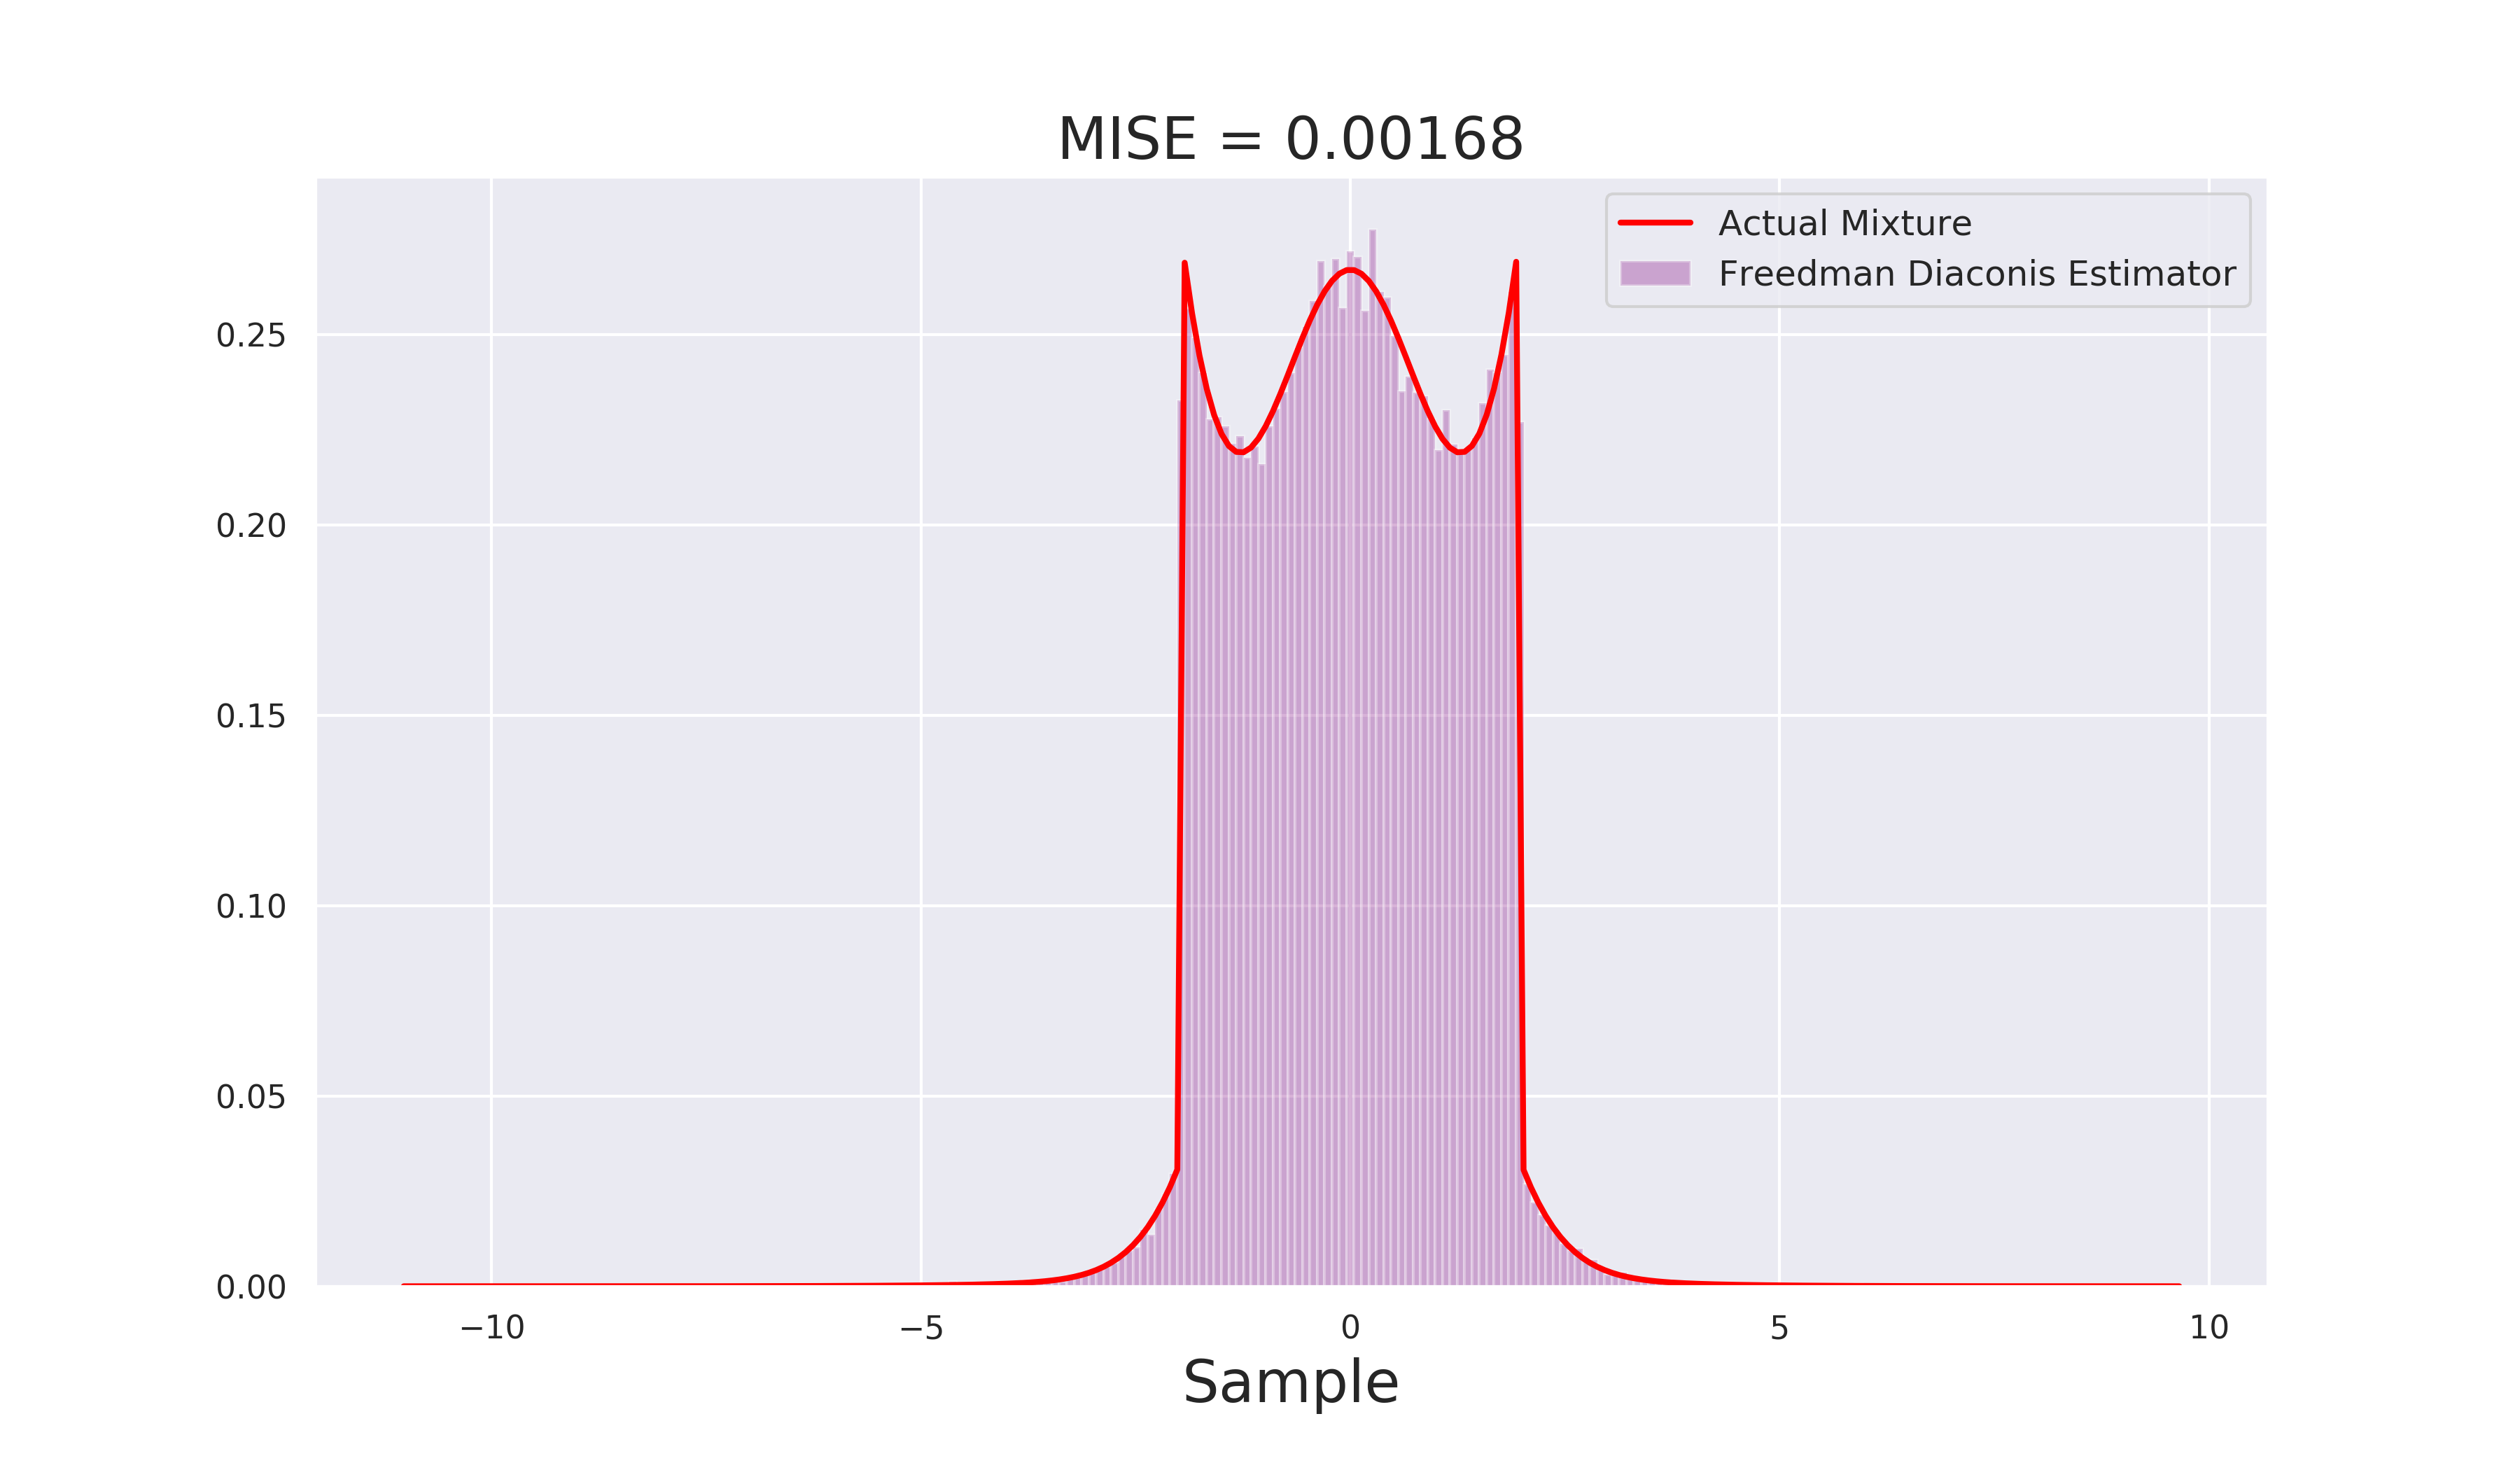
\includegraphics[width=\textwidth]{Images/Task2_1.png}
The following picture shows quality of different bin edge estimators \\
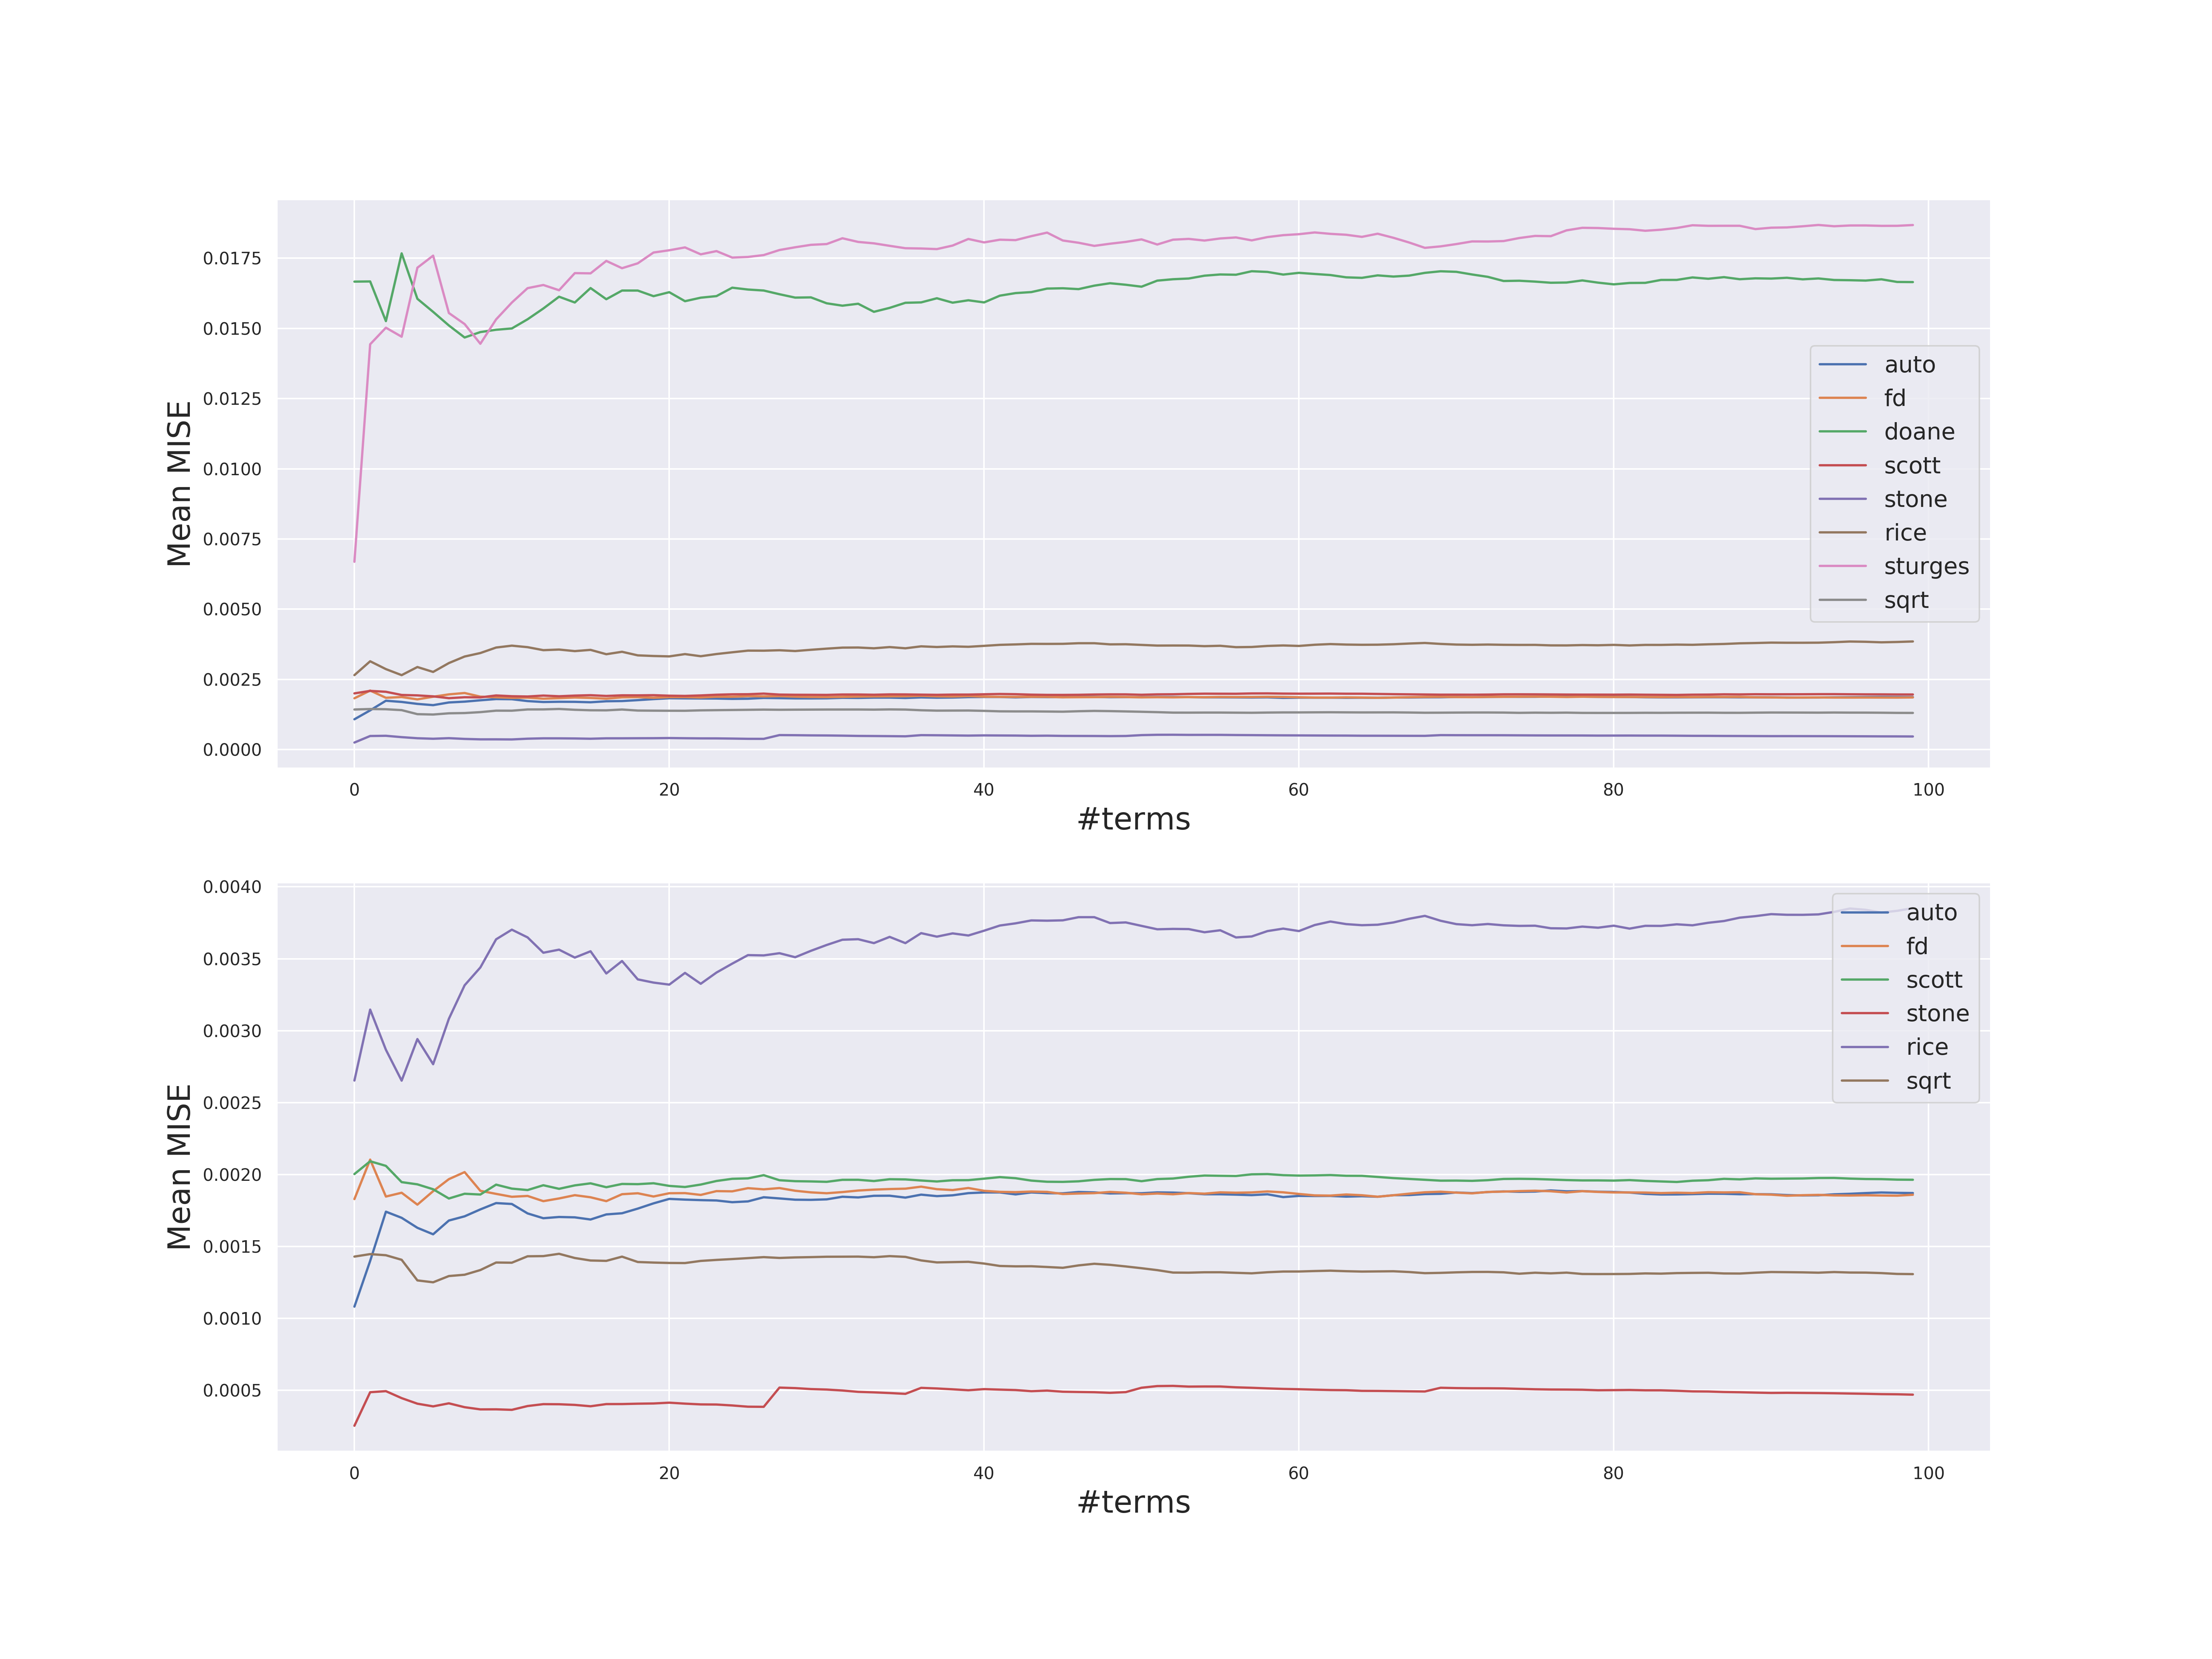
\includegraphics[width=\textwidth, height=9.5cm]{Images/Task2_2.png}\\
We can see that \textbf{Cross validation estimator (leave one out) a.k.a "stone"} gives us the best quality in sense of MISE. Use this \href{https://numpy.org/devdocs/reference/generated/numpy.histogram_bin_edges.html}{article} to get an acquaintance with other methods.

The following picture shows the optimal bandwidth \\
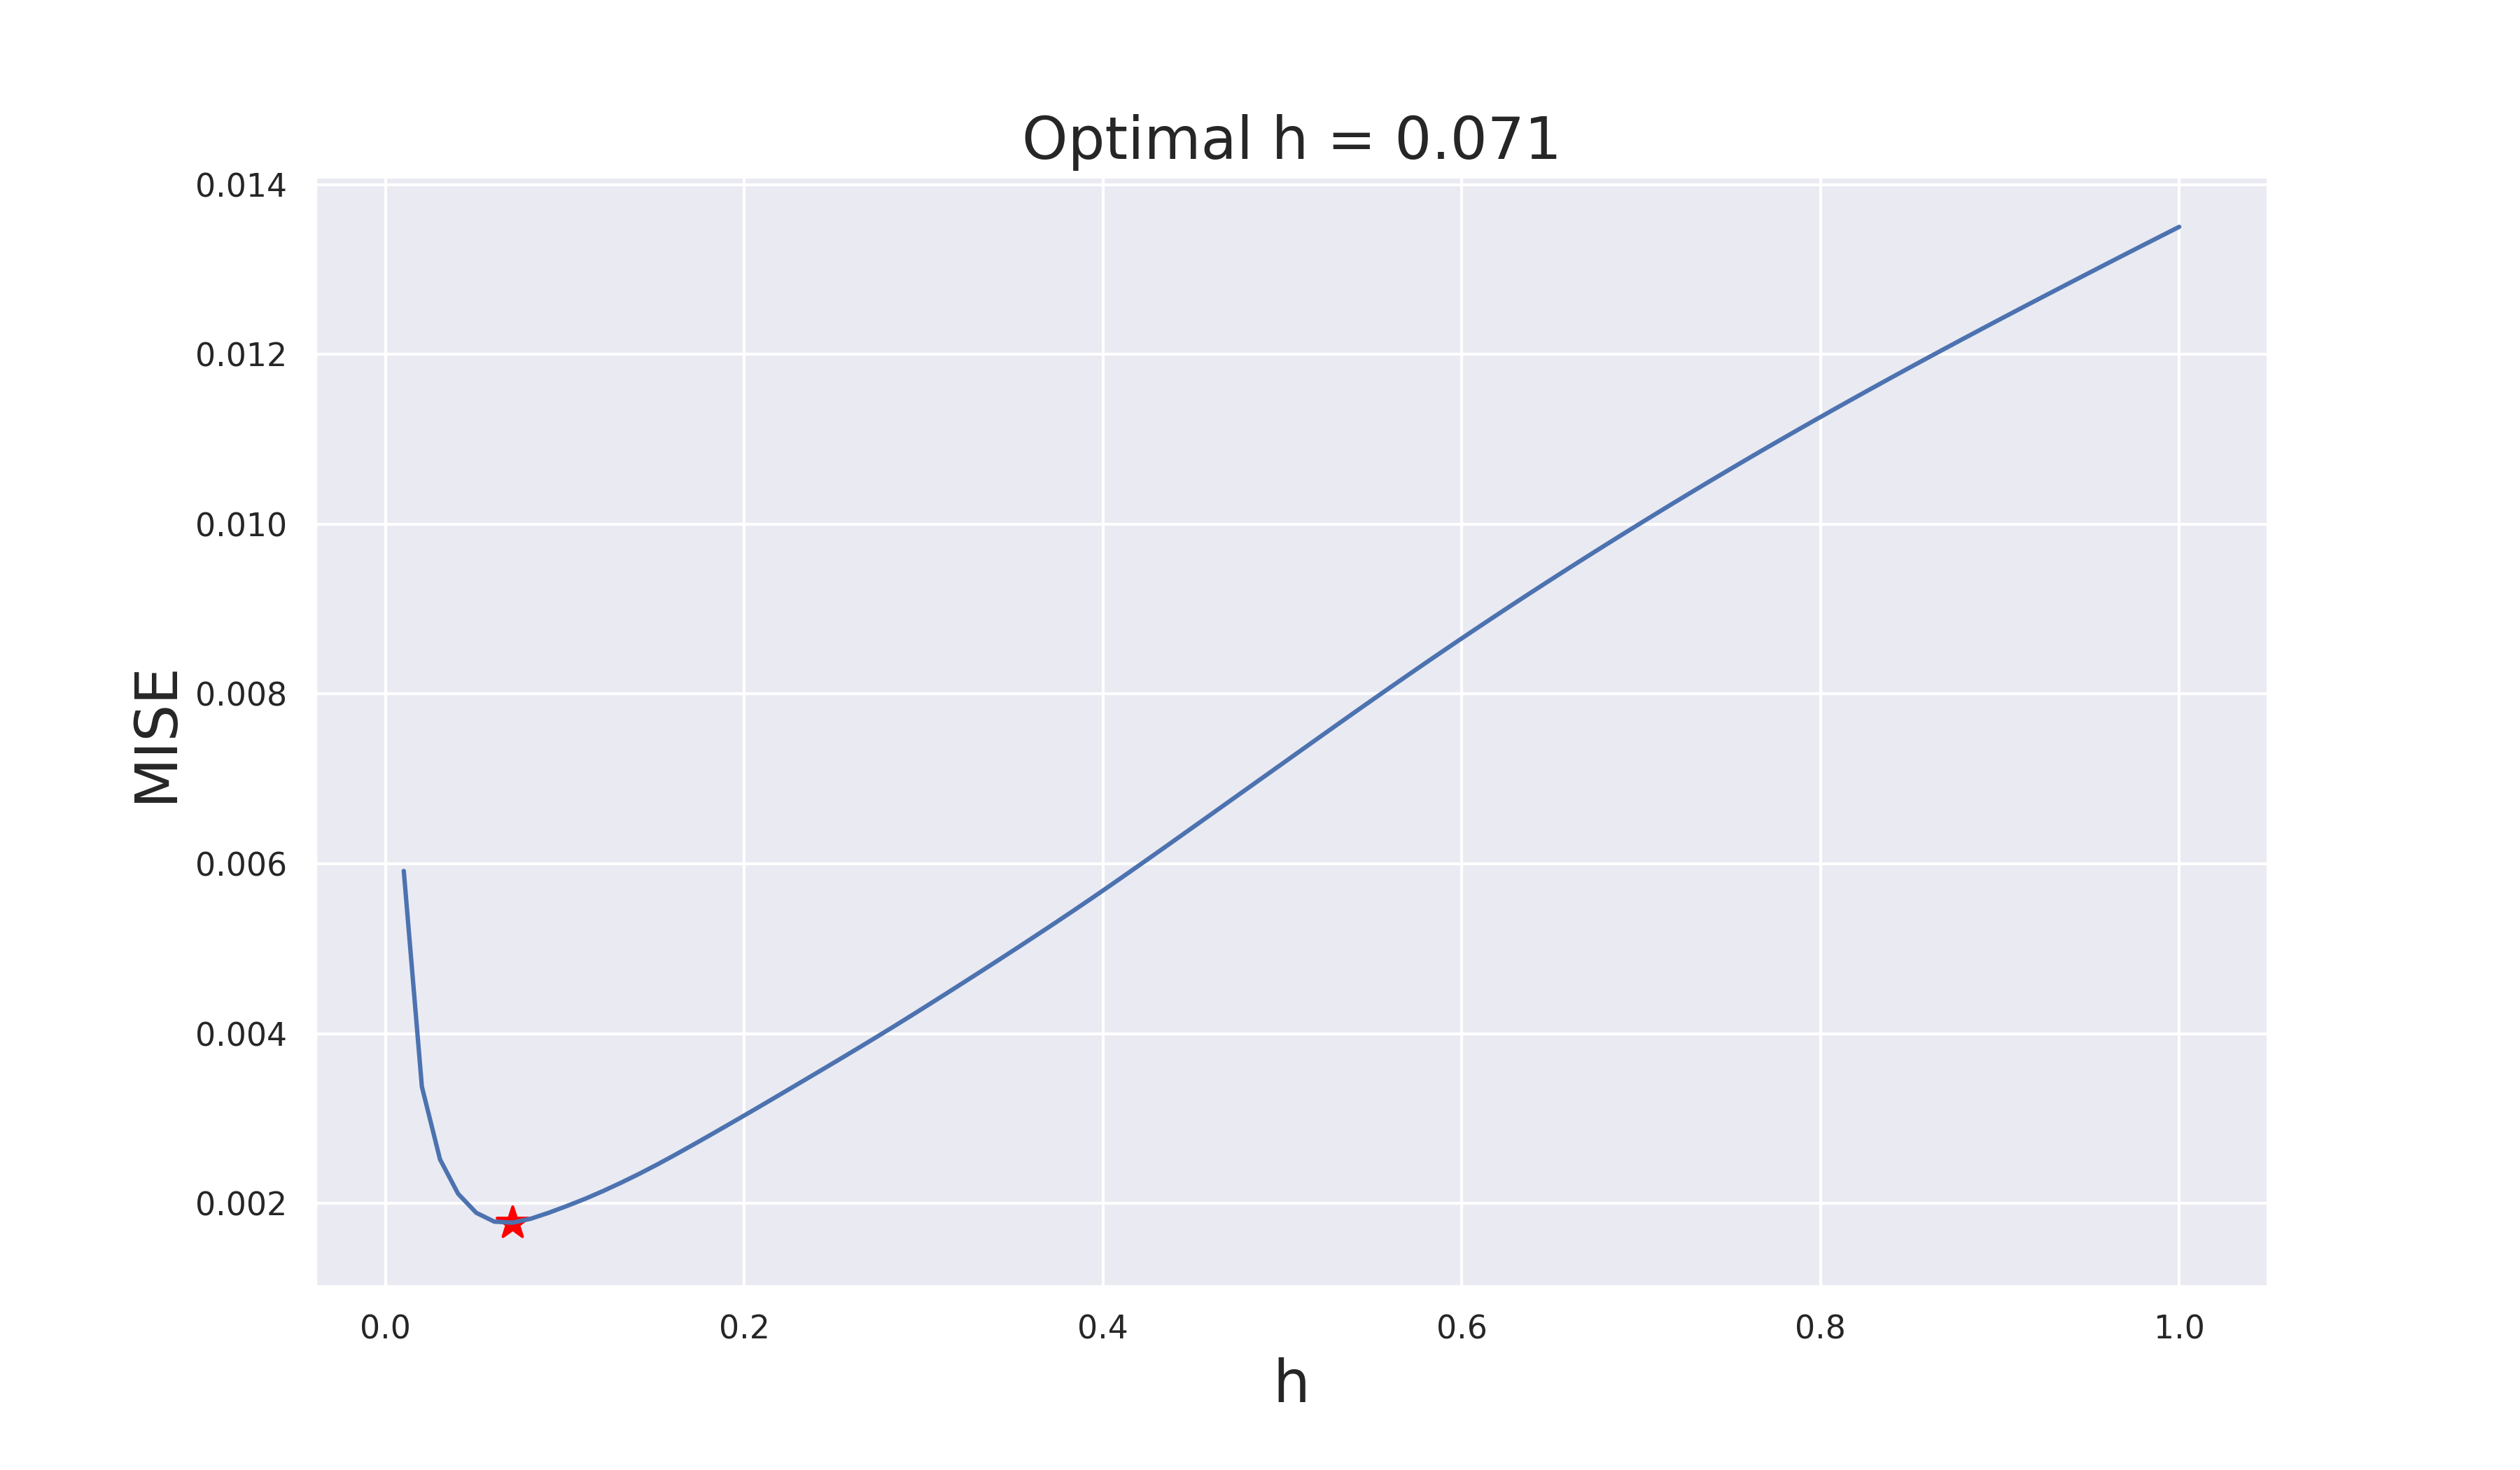
\includegraphics[width=\textwidth]{Images/Task2_3.png}
Now we have the finally result \\
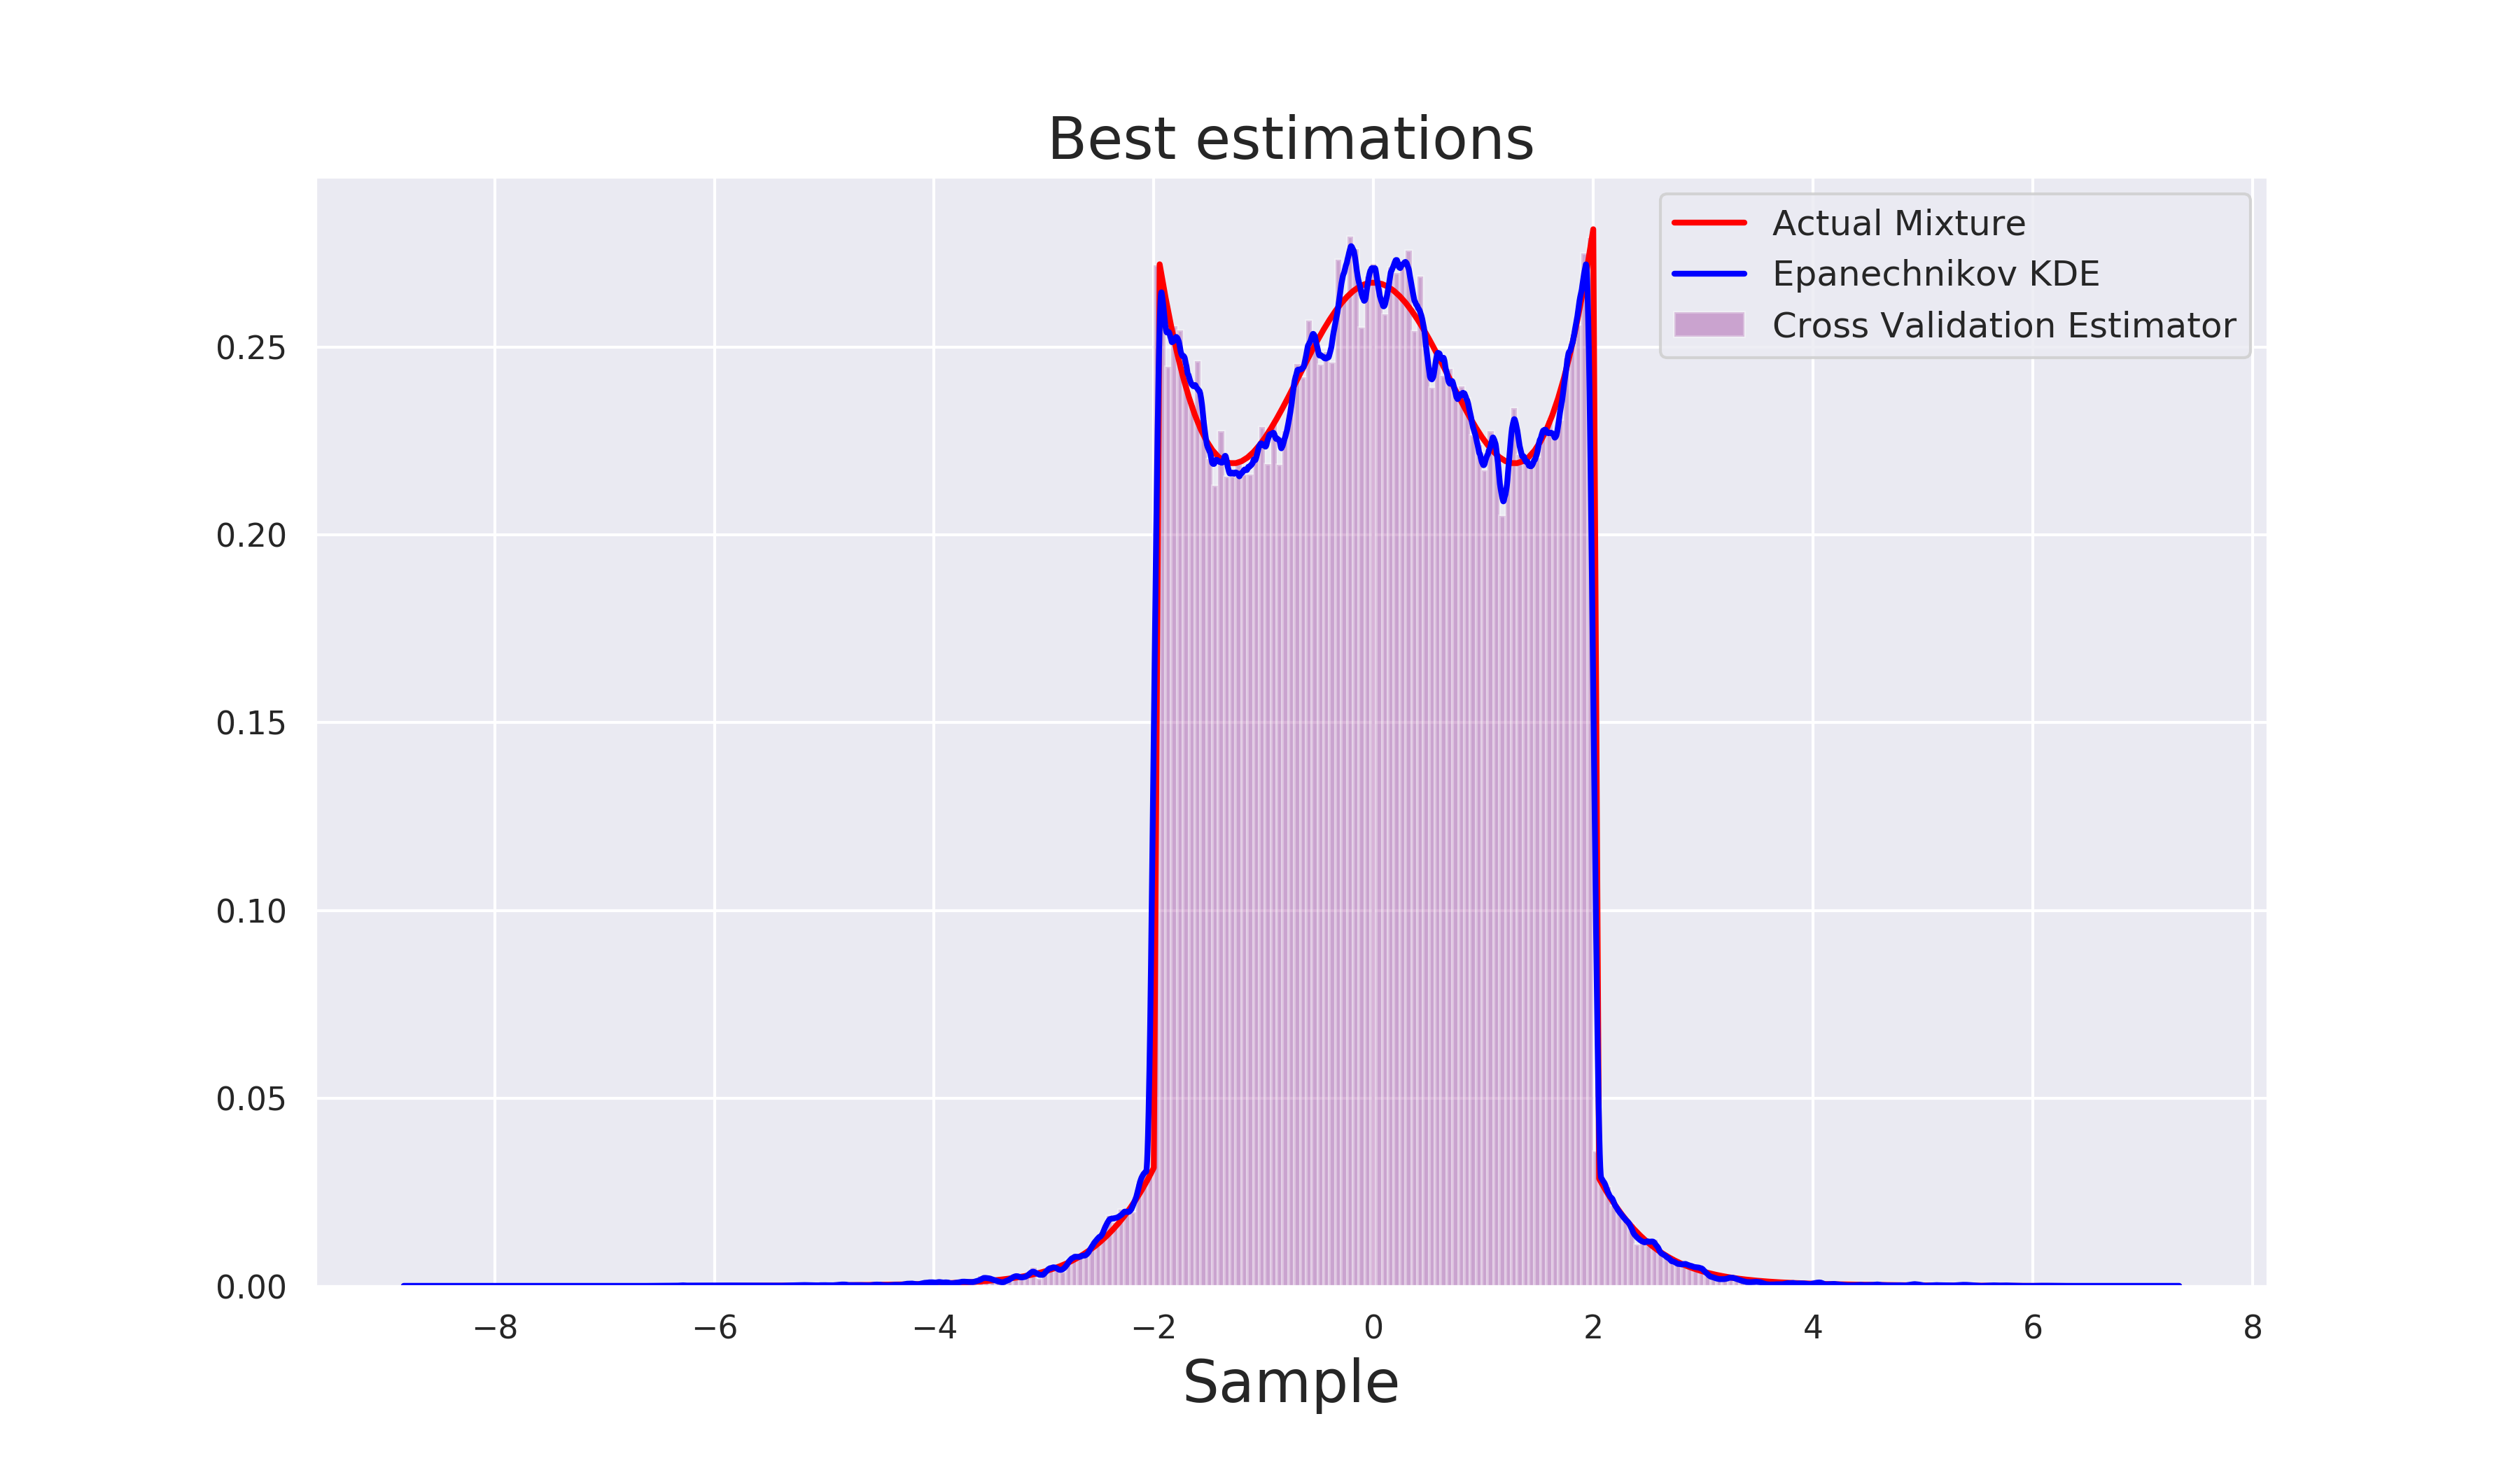
\includegraphics[width=\textwidth]{Images/Task2_4.png}


\section{Task 3}
\subsection{Theoretical solution}
Consider the mixture model. Suppose that the observations $X_i$ come from the next Gaussian mixture model
$$
\mathbb{P}(X_i = x) = p(x) = \sum \limits_{k=1}^K \pi_k p(x; \mu_k, \sigma^2_k)
$$
with $K$ mixture components. 
We want to maximize the likelihood function
$$
\mathbb{P}(X_1 = x_1, \ldots, X_n = x_n) = p(x_1, \ldots, x_n) = \prod \limits_{i=1}^n \sum \limits_{k=1}^K \pi_k p(x_i; \mu_k, \sigma^2_k) \rightarrow \max \limits_{\theta}
$$
where $\theta = \{ \mu_1, \ldots, \mu_K, \sigma_1^2, \ldots, \sigma_K^2, \pi_1, \ldots, \pi_K \}.$

Consider the log-likelihood function
$$
\mathcal{L}(\theta) = \sum \limits_{i=1}^n \log \left( \sum \limits_{k=1}^K \pi_k p(x_i; \mu_k, \sigma^2_k) \right) \rightarrow \max \limits_{\theta}
$$
which is supposed to be maximized by $\theta.$
It's hard problem to maximize $\log(\sum \ldots).$ But we can remember that we have the latent variables $Y_1, \ldots, Y_n,$ so we can rewrite the likelihood function as follows
$$
p(x_1, \ldots, x_n) = \prod \limits_{i=1}^n \sum \limits_{k=1}^K \pi_k p(x_i; \mu_k, \sigma^2_k) = \prod \limits_{i=1}^n \prod \limits_{k=1}^K \pi_k^{\mathbb{I}[Y_i = k|X_i = x_i]} p(x_i; \mu_k, \sigma^2_k)^{\mathbb{I}[Y_i = k|X_i = x_i]},
$$
where $ Y_i \in \{ 1, \ldots, K \}$ represents the mixture component for $X_i$ and $\mathbb{P}(X_i = x_i|Y_i = k)$ is the mixture component.

Since 
$$
\mathcal{L}(\theta) =  \sum \limits_{i=1}^n \sum \limits_{k=1}^K \mathbb{I}(Y_i = k|X_i = x_i) (\log \pi_k + \log p(x_i; \mu_k, \sigma^2_k))
$$ 
is a random variable, so expected value should be applied
$$
\mathbb{E}_{Y_i} \mathcal{L}(\theta) =  \sum \limits_{i=1}^n \sum \limits_{k=1}^K \mathbb{P}(Y_i = k|X_i = x_i) (\log \pi_k + \log p(x_i; \mu_k, \sigma^2_k)).
$$ 
Notice also that
$$
\gamma_k(Y_i) := \mathbb{P}(Y_i = k | X_i = x_i) = \dfrac{\mathbb{P}(X_i = x_i | Y_i = k) \mathbb{P}(Y_i = k)}{\mathbb{P}(X_i = x_i)} = \dfrac{\pi_k p(x_i; \mu_k, \sigma^2_k)}{\sum \limits_{k=1}^K \pi_k p(x_i; \mu_k, \sigma^2_k)}.
$$
Now we can differentiate $\mathbb{E}_{Y_i} \mathcal{L}(\theta)$ by $\mu_k, \sigma_k^2$ and get 
$$
\hat{\mu}_k = \dfrac{\sum \limits_{i=1}^n \gamma_k(Y_i) x_i}{\sum \limits_{i=1}^n \gamma_k(Y_i)},
$$
$$
\hat{\sigma}_k^2 = \dfrac{\sum \limits_{i=1}^n \gamma_k(Y_i) (x_i - \mu_k)^2}{\sum \limits_{i=1}^n \gamma_k(Y_i)}.
$$
To find $\pi_k$ we need to consider the next problem
$$
\begin{cases}
\sum \limits_{i=1}^n \sum \limits_{k=1}^K \gamma_k(Y_i) \log \pi_k \rightarrow \max \limits_{\pi_k \geqslant 0}, \\
\sum \limits_{k=1}^K \pi_k = 1.
\end{cases}
$$
The KKT theorem gives us the solution
$$
\hat{\pi}_k = \dfrac{1}{n} \sum \limits_{i=1}^n \gamma_k(Y_i).
$$
 
\section{Task 5}
To show that the minimum of the functional
$$
J(K) = \left( \int \limits_{- \infty}^{+\infty} K^2(x)dx \right)^{4/5} \cdot \left( \int \limits_{- \infty}^{+\infty} x^2 K(x)dx \right)^{2/5} \rightarrow \min \limits_{K \in \mathcal{C}}
$$
is attained on 
$$
K^*(x) = \dfrac{3}{4}(1 - x^2) \cdot \mathbb{I}[|x| \leqslant 1]
$$
where
\begin{equation}
\label{eq1}
\mathcal{C} = \left \{ K : K(x) = K(-x) \geqslant 0, \int \limits_{- \infty}^{+\infty} K(x)dx = 1 \right \},
\end{equation}
we are going to use the calculus of variations. 

Suppose $K^*(x)$ is a minimizer of the functional. Let $\varphi(x)$ be a continuous function such that $\varphi \in \mathcal{C}.$
Consider the variation $ \delta K^*(x) = \dfrac{K^*(x) + s \varphi(x)}{1 + s} \equiv K(x)$ that is also in the admissible set, e.g. $K \in \mathcal{C}.$

Denote
$$
g(s) = \left( \int \limits_{- \infty}^{+\infty} \left( \dfrac{K^*(x) + s \varphi(x)}{1 + s} \right)^2 dx \right)^{4/5} \left( \int \limits_{- \infty}^{+\infty} x^2 \left( \dfrac{K^*(x) + s \varphi(x)}{1 + s} \right) dx \right)^{2/5}.
$$ 
Hence $g(s)$ obtains a local minimum as $s = 0$ we have $g^{\prime}(0) = 0.$ 
Differentiate w.r.t $s$ we have
$$
g^{\prime}(0) = \dfrac{4}{5} \left( \int \limits_{- \infty}^{+\infty} (K^*(x))^2 dx \right)^{-1/5} 
\left( 2 \int \limits_{- \infty}^{+\infty} K^*(x) (\varphi(x) - K^*(x)) dx \right)
\left( \int \limits_{- \infty}^{+\infty} x^2 K^*(x) dx \right)^{2/5} +
$$
$$ 
+ \dfrac{2}{5} \left( \int \limits_{- \infty}^{+\infty} (K^*(x))^2 dx \right)^{4/5} 
\left( \int \limits_{- \infty}^{+\infty} x^2 (\varphi(x) - K^*(x)) dx \right)^{-3/5}
\left( \int \limits_{- \infty}^{+\infty} x^2 \varphi(x) dx \right) = 0.
$$
Some calculus give us 
$$
4 \left( \int \limits_{- \infty}^{+\infty} K^*(x) (\varphi(x) - K^*(x)) dx \right) 
\left( \int \limits_{- \infty}^{+\infty} x^2 K^*(x) dx \right) +
$$
$$ 
+ \left( \int \limits_{- \infty}^{+\infty}  (K^*(x))^2 dx \right)
\left( \int \limits_{- \infty}^{+\infty} x^2 (\varphi(x) - K^*(x)) dx \right) = 0,
$$
$$
\int \limits_{- \infty}^{+\infty} \varphi(x) \left[4 K^*(x) 
\left( \int \limits_{- \infty}^{+\infty} t^2 K^*(t) dt \right) + 
x^2 \left( \int \limits_{- \infty}^{+\infty}  (K^*(t))^2 dt \right) - \right.
$$
$$
\left. - 5 \left( \int \limits_{- \infty}^{+\infty} t^2 K^*(t) dt \right)
\left( \int \limits_{- \infty}^{+\infty}  (K^*(t))^2 dt \right)
\right] dx = 0.
$$
This equation holds for $\forall \varphi \in \mathcal{C},$ hence, $\forall x \in \mathbb{R}$
$$
4 K^*(x) 
\left( \int \limits_{- \infty}^{+\infty} t^2 K^*(t) dt \right) + 
x^2 \left( \int \limits_{- \infty}^{+\infty}  (K^*(t))^2 dt \right) - 5 \left( \int \limits_{- \infty}^{+\infty} t^2 K^*(t) dt \right)
\left( \int \limits_{- \infty}^{+\infty}  (K^*(t))^2 dt \right) = 0.
$$ 
Rewrite the last equation as following
$$
K^*(x) = - \dfrac{\left( \int \limits_{- \infty}^{+\infty}  (K^*(t))^2 dt \right)}{4\left( \int \limits_{- \infty}^{+\infty} t^2 K^*(t) dt \right)} x^2 + \dfrac{5}{4} \left( \int \limits_{- \infty}^{+\infty}  (K^*(t))^2 dt \right).
$$
It gives us the next tip $K^*(x) = -ax^2 + c$ where $a \geqslant 0, b \geqslant 0$ are parameters which can be found. 
But for convergence of the integrals we must modify $K^*(x)$ as following
$$
K^*(x) = (-ax^2 + c) \mathbb{I}[|x| \leqslant \alpha], ~ \forall \alpha > 0.
$$
Using $\int \limits_{-\infty}^{+\infty} K^*(x)dx = 1$ we solve the next system of equations
$$
a = \dfrac{\left( \int \limits_{- \infty}^{+\infty}  (K^*(t))^2 dt \right)}{4\left( \int \limits_{- \infty}^{+\infty} t^2 K^*(t) dt \right)}, ~ c = \left( \int \limits_{- \infty}^{+\infty}  (K^*(t))^2 dt \right).
$$
As a result we have
$$
a = \dfrac{3}{4 \alpha^3}, ~ c = \dfrac{3}{4\alpha}.
$$
We can choose $\alpha = 1$ and finish the proof.
\end{document} 